% Chapter Template

\chapter{Results} % Main chapter title

\label{Chapter3} % Change X to a consecutive number; for referencing this chapter elsewhere, use \ref{ChapterX}

%----------------------------------------------------------------------------------------
%	SECTION 1
%----------------------------------------------------------------------------------------
\section{Setup}
In this paper, we discussed a pipeline implemented using python then C\# and Unity’s real time development platform, as the visualization engine. We ran a Levelset 4, FDS simulation, set to output plot3D files every 0.5 seconds on a 20m x 20m x 20m mesh, containing voxels 0.2m x 0.2m x 0.2m in size, with open boundary conditions. The simulation was 100 seconds in length with a ground fire igniting ten seconds into the simulation, with a wind of 5.6 m/s originating from the south west (215\textdegree) and trees evenly distributed on the mesh.  [Figure \ref{fig:CFDTopDown} shows a top down view of our visualization rendered in SmokeView] \par
[Github link to fds file?]\par
\section{Analyses}
The total run time for this simulation took 252 (4 Hours 12 Min ) minutes to complete running 4 cores of an i7 4790k in parallel. While calculations we discussed in this paper were able to complete in three minutes, with no parallelization at the moment. Additionally, the size of the CFD output files was 5.0 Gigabytes, while the saved data needed for full Virtual Reality using our methodology is 28.9 Megabytes, a 99.4\% reduction in file size. When visualized inside of unity using a HMD ( HTC Vive and HTC Vive Pro was used during testing) were able to average 15-30 frames per second with a resolution of 1440 x 1660 pixels per eye, with the lowest frame rate during the transition between timesteps.
\begin{figure}
\centering
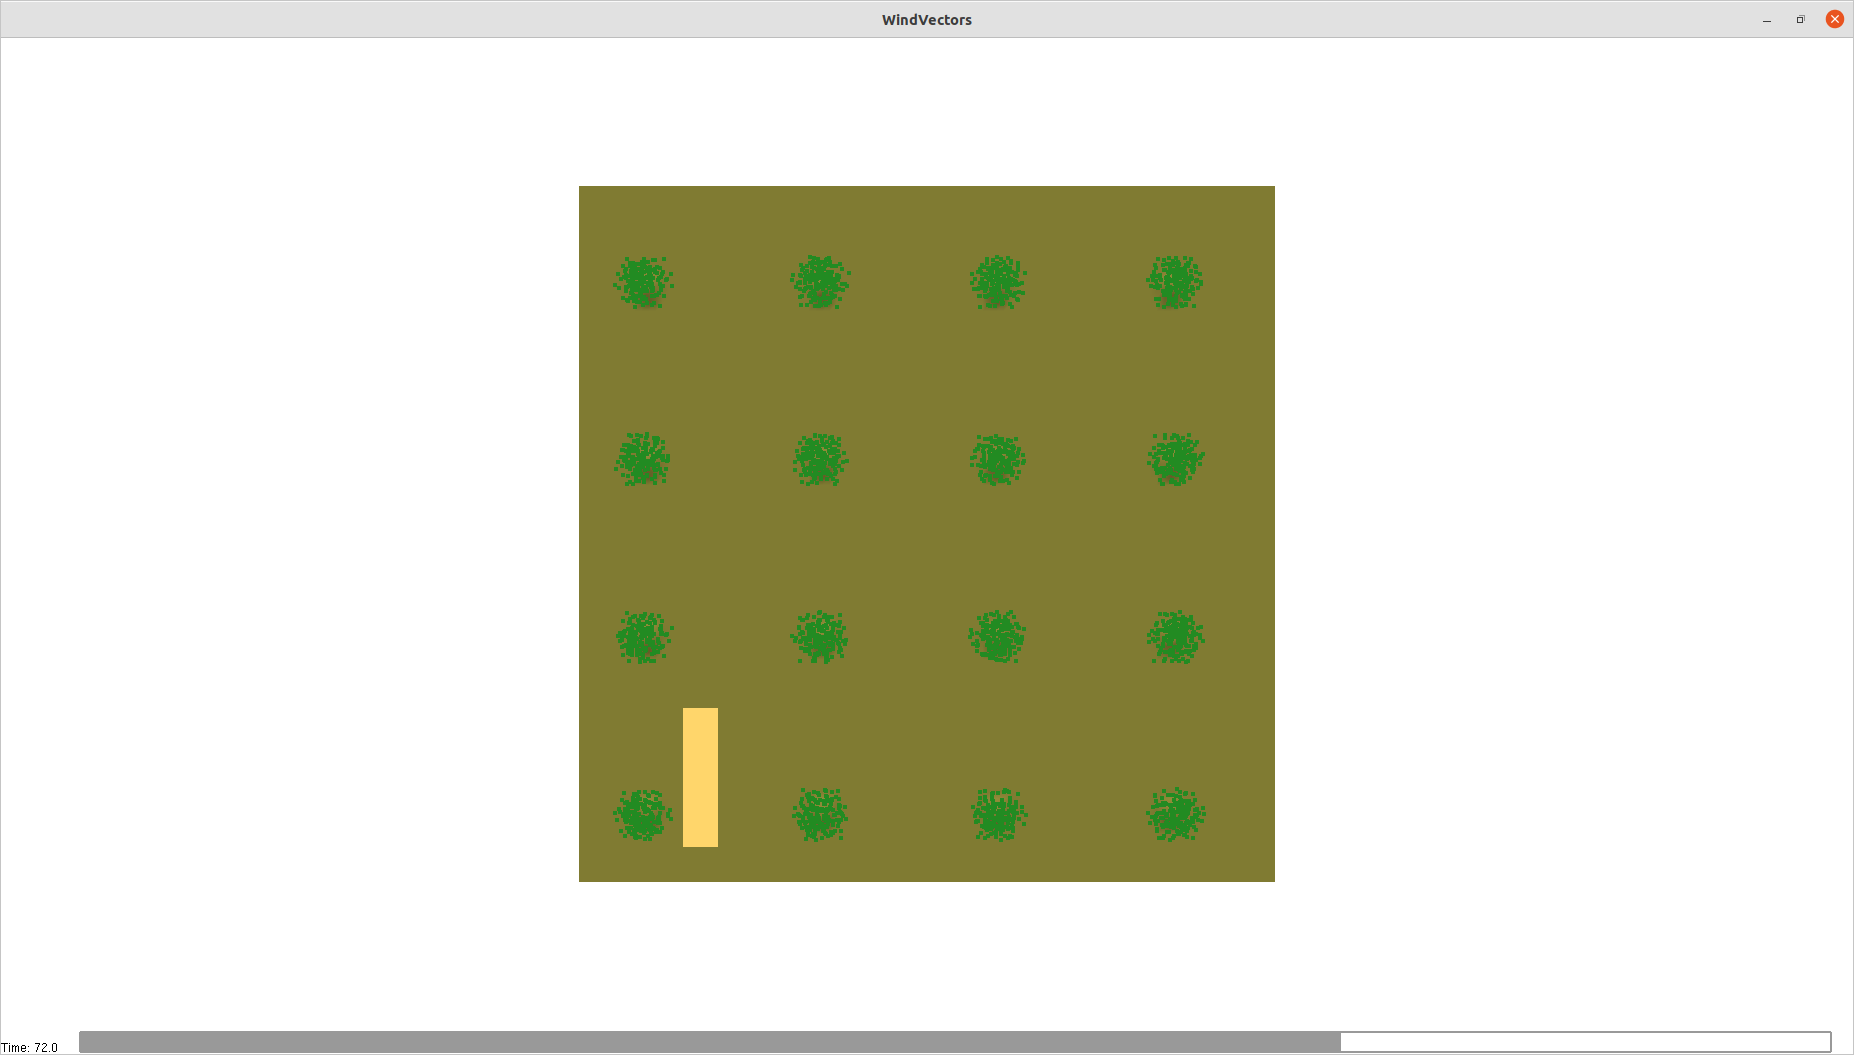
\includegraphics[scale=.1]{Figures/fdsPartTopView.png}
\decoRule
\caption[CFD Simulation]{A top-down view of the CFD simulation}
\label{fig:CFDTopDown}
\end{figure}